\documentclass[12pt,a4paper,oneside]{book} 
%scrbook book report

\usepackage{multirow}
\usepackage{graphicx}
\usepackage[table]{xcolor}
\usepackage{float}
%\usepackage{color}
%\usepackage{subfigure}
\usepackage{seecs}
%\usepackage{color}
%\usepackage{colortbl}
%\usepackage{soul}
%\usepackage{listings}
%\lstloadlanguages{Java,XML}
%\lstset{frame=lines}
%\usepackage{astron}
%\usepackage{xspace}
%\usepackage[leqno]{amsmath}
%\usepackage{hyperref}
%\usepackage{sfmath}
%\usepackage{setspace}
\usepackage{cite}
\definecolor{lightgray}{gray}{0.9}


%\usepackage{amsmath,amssymb,amsthm,paralist}
%% Include other packages you wish to use except setspace.
%% That package is loaded automatically.
%% IMPORTANT: Load only those packages you know you will use.
%% Some packages can cause conflicts resulting in improper formatting.
%\usepackage{graphicx}
%\usepackage{subfig}
%\usepackage{latexsym}
%\usepackage{url}
%%\usepackage{soul}  % package for strikeout \st{}
%\usepackage{algorithm}
%\usepackage{algorithmic}
\usepackage{cite}
\renewcommand{\baselinestretch}{1.5}
\setcounter{secnumdepth}{3}


\title{Student Degree Record Exchange Standard}
%\subtitle{An optional sub-title, usually not used at NUST}

\author{Umair Anwar}
\regno{2011-NUST-MS PhD-IT-049}
\degree{\MSIT} 
% Argument pptions for \degree{_____}:
% \BSIT for Bachelor of Science in Information Technology (BS IT)
% \BSCS for Bachelor of Science in Computer Science (BS CS)
% \BICSE for Bachelor of Engineering in Information and Communication Systems (BE ICS)
% \BEE for Bachelor of Engineering in Electronics (BE Electronics)
% \MSIT for Masters of Science in Information Technology (MS IT)
% \MSCSE for Masters in Communication Systems Engineering (MS CSE)
% \MSCCS for Masters in Computer and Communication Security (MS CCS)
% \MSEE for Masters of Science in Electrical Engineering (MS EE)

\adviser{Dr. Sharifullah Khan}
\adviserAffiliation{Department of Computing}

\date{July 2015}

%\setcounter{tocdepth}{2}
 %\setstretch{1.1}
 %\linespread{1.1}

\begin{document}
\maketitle

\evaluationcommitteeapproval{Dr. Hamid Mukhtar}{Dr. Sarah Shafiq Khan}{Mr. Mujtaba Haider}

\chapter*{Abstract}

 Bologona process aimed to ease the mobility of students across Europe. Hence, efforts were put developing standards and proposing suitable architectures that fit all across Europe. Inspired by this, the mobility project tried to gather and reuse all the work previously done in related areas. Mobility reused the vocabularies, ideas and focused on the mobility of students. However, it created an opportunity for a semi-automated mapping tool for mapping proposed standard to the heterogeneous schema of different institutes. It lacks enough vocabulary to cover exchange of information for some educational certificates in Pakistan. \\
 
 We suggest a prototype infrastructure that provides more control and improves this exchange of information between partaking institutes by covering more detailed vocabulary. The term infrastructure includes both the architecture and our proposed standard (DRESS). We avail the opportunity that The Mobility Project provided and suggest a mapping tool that semi-automatically create mappings between our standard and the heterogeneous data-sets of different partaking institutes. \\
 
To evaluate this research, we created a test-bed environment and validated the proposed standard XML schema definitions against the generated XML documents using different evaluation techniques. 

%---------------------------------------------------------------------
\certificateoforiginality
%---------------------------------------------------------------------
\chapter*{Acknowledgment}
All gratefulness and wonderfulness to {\bfseries ALLAH} and with His blessings, I am in good health and he gave me the ability to complete this work. I pray for more of Allah's blessings. It would not be possible without the efforts that were made by my {\bfseries parents} for supporting me during this duration and throughout my life. \\

I am truly thankful to my supervisor {\bfseries Dr. Sharifullah Khan} for his guidance and who had been a great coach. I want to express my gratitude towards him for believing in me and facilitating me for the completion of this work. I appreciate {\bfseries Dr. Hamid Mukhtar}, {\bfseries Dr. Sarah Shafiq Khan} and {\bfseries Mr. Mujtaba Haider} for suggesting and supporting me. \\

I am thankful to all my colleagues, co-workers and contributors who were supportive in completing this research.

\begin{flushright} \textbf{Umair Anwar} \end{flushright}
%---------------------------------------------------------------------

\tableofcontents
%
%\printnomenclature{2.5cm}
%\nomenclature{DCF}{Distributed Coordination Function}
%
%
\chapter*{List of Abbreviations}

\begin{table}[h]
   % increase table row spacing, adjust to taste
    \renewcommand{\arraystretch}{1.3}
    \label{table:table1}
     \begin{tabular}{ll}
        \hline\hline
        % inserting double-line
            {\bfseries Abbreviations} & {\bfseries Descriptions} \\
            \hline                                      % inserts single-line
            DRESS & Document Record Exchange Standard of Students  \\
            SCHAC & Schema for Academia  \\
            LDAP & Lightweight Directory Access Protocol \\
            FVUSPEC & Finnish Virtual University Specifications  \\
            MLO & Meta-data for Learning Opportunities  \\
            WSDL & Web Service Description Language  \\
            EHEA & European Higher Education Area  \\
            ECTS & European Credit Transfer and Accumulation System  \\
            EA & Exchange Agreement  \\
            NQF & National Qualifications Framework  \\
            EQF & European Qualifications Framework  \\
            XSD & XML Schema Definition  \\
            ECV & Europass Curriculum Vitae \\
            ELP & Europass Language Passport \\
            
            \hline                          % inserts single-line
    \end{tabular}
\end{table}

\listoffigures
\listoftables
% \lstlistoflistings

\resetpagenumbering
%---------------------------------------------------------------------

\chapter{Introduction}\label{ch-intro}
%-----------------------------------------------

With time passing, the exchange of official and legal documents digitally is getting more and more importance. In near future, it will be inevitable to transform our systems to facilitate this change. Same is the case with the exchange of educational certificates between different partaking institutes and authorities. Its importance can be imagined by the number of students and institutes involved. \\

In 1999, it was decided in Bologna declaration to create European Higher Education Area which facilitate to standardize the exchange of information across Europe. Alone in Europe, more than four thousands partaking institutes with more than two million students were involved in this process in academic year 2009-2010. \\

In April 2015 Bureau of Statistics Pakistan published statistics about Pakistan's population with different levels of education \cite{Level of Edu}. There are 1,712,308 people having education of BA/BSc \& Equivalent and 618,937 people with MA/MSc \& Equivalent or Above education. \cite{Edu Stat} \\

Ministry of Federal Education and Professional Training and USAID published detailed report on Pakistan Education Statistics 2010-2011 \cite{Edu Stat}. We are mentioning the higher education enrollment statistics from this report to get an idea for need of this research. According to this report there are 135 higher education institutes with total enrollment of 1.108 million. This number includes all bachelors, masters or above enrollments. It is also worth mentioning that 1,558 degree colleges have an enrollment of 0.431 million students. \\ 

According to Pakistan Education Statistics 2013-2014 report there are 161 higher education institutes with total enrollment of 1.595 million. This number includes all bachelors, masters or above enrollments. It is also worth mentioning that 1086 degree colleges have an enrollment of 1.336 million. \cite{Edu Stat2}\\

The statistics we collected from Pakistan Education Statistics reports are represented in table \ref{tab:pakedustats}. These statistics suggest that the number of students are increasing. Although the number of degree colleges has decreased but the number of students have almost tripled in degree colleges from 2010 to 2014. The number of enrollments in universities have also increased. These statistics signify the importance of this research.

\begin{table}[!tbh]
%\renewcommand{\arraystretch}{1.5}
\caption{Statistics from Pakistan Education Statistics Reports}
\label{tab:pakedustats}
\centering
\begin{tabular}[width=\columnwidth]{|p{1.3in}|c|c|c|c|c|}
\hline
Academic Year               	& Enrollments in Colleges		& Enrollments in Universities\\
\hline
2010-2011 	    	& 0.431 million					& 1.108 million \\
2013-2014	    	& 1.336 million 				& 1.595 million \\
\hline
\end{tabular}
\end{table}

It is a well established fact that more and more systems are digitized every year. The educational institutes are also making their record digital and this trend is increasing. For example, more and more universities are implementing electronic student information systems to keep student courses and credit record. However, the documents often called degrees/certificates issued by these autonomous bodies are still exchanged in paper form.  \\

This manual approach of exchanging physical documents and re-entering the data again manually in digital or physical form by people is error prone and exhaustive. As a result the local data-sets of these autonomous bodies has different record for the same individual. \\

This creates an opportunity for a common data-exchange standard which bring a common ground for the exchange of information. To resolve the issues facing in manual exchange of documents, the institutional systems must talk to each other using a common standard. This would make the entire process more dependable and less error prone. \\

This research digs into the currently adopted solutions, standards and the new research in the area of student mobility and exchange of official documents related to students. It suggests a prototype infrastructure including data format and the architecture to exchange degree records digitally. \\

Each institute is an autonomous body maintaining its data separately. The schema of the data is different in different institutes. To exchange documents, partaking institutes must implement web-services based on our proposed architecture and Document Record Exchange Standard for Students (DRESS). We will use only DRESS in rest of the thesis. This approach is very time consuming, inefficient, and error prone. This provides us another  opportunity to suggest a tool that maps these different types of databases schema from different institutes to DRESS. \\

To handle the different levels of heterogeneity, we came up with a mapping tool which semi-automatically maps institutes data-sets to our proposed standard and creates web-services to access their data. \\

The remaining chapter is sorted out as this; In Section 1.1, we explain the problem Statement. In Section 1.2, we discuss what this research has contributed. In Section 1.3, we explain how this research is organized into chapters.

\section{Problem Statement}\label{s-problem_statement}

The existing standards that are used for exchanging educational certificates partially cover attributes that are required for the exchange of these documents. These are developed mostly as part of other projects and thus only focusing in this domain partially. Hence, most of these lack some basic attributes that are necessary for a standard to be usable. \\

We take a step and put an effort in suggesting a standard that is generic, reusable, extendable and based on technologies that are platform independent and widely usable accompanying tools that make it easy to implement and use. So, our formal problem statement becomes; \\   

"To propose a document record exchange standard for students that enables the partaking institutes to exchange educational certificates while hiding the heterogeneous details. The proposed standard must reuse the ideas already suggested in existing standards and must be generic, extendable, reusable and easy to use. The standard must accompany the tools that make it easily usable." 

\section{Contributions}\label{s-contributions}
This research made following contributions;

\begin{itemize}
\item
It explored existing standards and tools that are available for the exchange of educational certificates. It identified the attributes that are lacking in these standards. 
\item
It suggested DRESS, a new educational certificates exchange standard, that reuses the ideas in previous standards and cover some attributes that were missing in these standards.
\item
It suggested a mapping tool that maps different heterogeneous schema to DRESS semi-automatically.
\item
It suggested an algorithm for the exchange of information over the proposed architecture using DRESS.

\end{itemize}


%\subsection{Motivation}

%\begin{itemize}
%\item

%\item
%Finding 2.
%\end{itemize}

\section{Goals}\label{s-goals}

\begin{itemize}
\item
Propose a generic and extendable standard for the exchange of educational certificates with well defined vocabulary.
\item
Suggesting a suitable prototype architecture for the exchange of educational certificates such that 
every data owning entity is the owner of its own data to build trust and have built-in control for authenticity.
\item
Implementation of a mapping tool to ease mapping of heterogeneous schema with our proposed standard DRESS.
\end{itemize}

%\subsection{Challenges}\label{s-challenges}

%\begin{itemize}
%\item
%sdfs
%\item
%Finding 2.
%\end{itemize}

\section{Thesis Organization}\label{s-thesis-organization}

Let us now discuss how we have organized the remaining research in chapters: \\

In Chapter 2, we go through the literature review. We discuss the work that has already been done for exchanging student information. We look into the already existing standards, a few implementations and related projects. We will go deep in details in this section, to understand the ideas and technologies that are already in use. \\

In Chapter 3, we discuss the business process in detail using sequence diagrams and define the functional and non-functional requirements.  \\

In Chapter 4, the proposed architecture and design are discussed in detail. \\

In Chapter 5, our proposed standard "DRESS" is presented. We discuss its vocabulary and the possible values. \\

In Chapter 6, we discuss the implementation and the test-bed environment we created. In this chapter, we also evaluate whether the goals are achieved. \\

In Chapter 7, the research work is concluded and possible future work is presented.

\chapter{Literature Review}\label{ch-work}

There already exists a few standards and practices identified with exchanging degree or courses record. It is important to go through these, before proceeding onward to the new standard and the architecture we are proposing. We will review what these standards cover and what we can reuse. 

\section{Bologna Process}

It intends to make European educational framework of standards engaging different countries in Europe to compare, contrast and make compatible their educational systems. \cite{bologna process} \\

To improve the mutual recognition of degrees and programs, education ministers from 29 countries signed bologna declaration in 1999. Other partaking countries joined the program later. \cite{improvement bologna process} Bologna process is quite often named as European Higher Education Area (EHEA). EHEA focuses on transferal and convergence adaption by 46 countries. This process benefits Europeans and it has its significance for other educational institutes and communities. The significance of EHEA is due to these reasons;

	\begin{enumerate}

		\item The leading role of European institutes,

		\item the lessons that are learned in the implementation of the framework of standards, and
	
		\item the practices adopted guide the educational communities around the world.

	\end{enumerate} 

	2010 was marked as the deadline across Europe for implementing the agreed specifications. \cite{EHEA} To meet the 2010 deadline, Spain started to implement the convergence of undergraduate engineering degrees that conformed EHEA in 2008. This standardization provided some opportunities for mobility and unified measurements. \cite{EHEA}

\section{Qualifications Exchange Standards}

    \subsection{European Qualifications Framework}
    EQF is an agreed reference framework that helps participating countries to compare national qualifications and make them more clear, readable and understandable across Europe. The point is to advance mobility of workers and learners. This was settled upon by European universities in 2008 to relate their national qualifications to EQF. The new qualifications from 2012 carry a reference to suitable EQF level. \\

    EQF comprises of eight reference levels, each showing what a learner knows and has the capacity to understand it. National qualifications of the partaking countries identify and relate with these eight levels raging from basic (level 1) to advanced (level 8) as shown in figure ~\ref{fig:EQF}. This simplifies qualification comparison in partaking countries supporting mobility of learners and empowering them to not repeat what they have already learned. \\

\begin{figure}[!hbp]
  \centering
  \includegraphics[width=14cm]{eqf.png}
  \caption{EQFs against NQFs \cite{MAPQFTOOL}}
  \label{fig:EQF}
\end{figure}

    EQF concentrates on learning results as opposed to concentrating on learning inputs. It covers all types of education including professional, vocational and school education. It tries to validate formal and in addition informal education. 

    \subsection{Europass}
    Collection of five documents which intend to ease mobility when seeking employment across Europe. These include the Curriculum Vitae, the Language Passport, the Mobility, the Diploma Supplement, and the Certificate Supplement. One can fill himself the Curriculum Vitae, and the Language Passport but the rest of the documents are issued by the related authorities. It follows a standard template format system, a layout. Same format helps to achieve neutrality and transparency while presenting one's skills. \\

    The motto as mentioned on the Europass website's homepage is as follows; \\
    "Five documents to make your skills and qualifications clearly and easily understood in Europe" \cite{Europass Web} \\

    Europass has defined XML schemas for CV and Language Passport. The documents can be exported in XML format when created on Europass. These exported XML documents can be imported to Europass and converted to HTML, PDF, Microsoft Word or ODT templates. \\

    Europass specifies JSON schema according to Internet Engineering Task Force's JSON specifications draft. The europass JSON vocabulary is close and similar to europass XML schema. The JSON objects for europass documents (CV and Language Passport) can be validated using Europass JSON validator. \\

    All these documents have some common XML schema attributes which describe document type, printed preferences. \\

    Europass does not explain details related to degrees or educational certificates in XML certificate. 

        \subsubsection{Europass Curriculum Vitae}
        Europass Curriculum Vitae (ECV) is a template which one can create online and it can be exported in XML format. The ECV XML schema contains vocabularies related to document type, printing preferences, personal details, contact details, skills, and educational degrees and institutes. The XML vocabulary related to degree details is very little only to cover the scope of a CV. 

        \subsubsection{Europass Language Passport}
        Europass Language Passport (ELP) is a template. One can create it online and export it in europass xml format. It contains XML vocabulary related to language skills and the scale of six values to score proficiency. 

    \subsection{Schema for Academia \cite{SCHAC 1.5.0}} 
    The need for the inter-exchange of information between institutes across Europe has highlighted the importance of common attributes for this exchange to take place. Schema for Academia (SCHAC) is the result of the attribute coordination between different institutes. It plans to define and advance common attributes in the field of higher education to encourage data-exchange between institutions. It does not plan to supplement different the national schemas, rather it suggests a coordinated framework on top of the different national schemas. \\
    
    Schema for Academia (SCHAC) describes vocabulary related degrees and courses. The schema is not technology dependent and written for LDAP (Lightweight Directory Access Protocol). It aims at promoting a common framework to inter-exchange data between educational institutes. It defines attributes that describe individuals and their LDAP profile. \\
    
	It is a collection of schemas which can be classified into following categories;
\begin{itemize}
\item
Personal Characteristics
\item
Location Information
\item
Student Information
\item
Employee Information
\item
Linkage Identifiers
\item
Administration Information
\item
Confidentiality (Visibility)
\item
Authorization, Entitlements
\item
Group-related Attributes
\end{itemize}

	SCHAC has a clearly defined meta-information for defining an attribute. To discuss the ideas  used by SCHAC, let us look in detail the schacGender attribute as an example shown in Table \ref{tab:schacGender}. It uses ISO-standards where-ever possible. In schacGender attribute, it is using values from ISO-5218. However, it lacks hierarchy which prevents from reuse-ability and it can be considered its disadvantage. \\
	
\begin{table}[!tbh]
%\renewcommand{\arraystretch}{1.5}
\caption{Example of SCHAC attribute: schacGender \cite{SCHAC 1.5.0}.}
\label{tab:schacGender}
\centering
\begin{tabular}[width=\columnwidth]{|p{1.3in}|c|c|c|c|c|}
\hline
Name               	& schacGender \\
\hline
Description 	    & Male or Female, specify the legal gender	\\
Format	    		& 0 - Not Known, 1 - Male, 2 - Female, 9 - Not Specified \\
Values				& Single \\
References	        & ISO-5218	\\
Example	            & schacGender = 1	\\
\hline
\end{tabular}
\end{table}

It is also worth mentioning that SCHAC has a category student information for curriculum, major and degree but no attribute is defined. This is because SCHAC is not completed till now and it is in progress. 

    \subsection{Dublin Core}
    The Dublin core is a simple meta-data standard consisting of set of elements to describe information resources on the network. There are two type of elements; simple and qualifiers. It has 15 simple elements and qualifiers which have additional three elements namely Audience, Provenance and RightsHolder. Qualifiers help in resource discovery. \cite{The Mobility Project} 

\section{European Learner Mobility}
Some related work has been done recently and systems have been proposed based on the above mentioned standards. These are "The Mobility Project" and "The REST Mobility" projects. 

    \subsection{The Mobility Project}
    It aimed to provide a platform and infrastructure for exchange of electronic data exchange between educational institutes. Infrastructure includes data format, architecture and the prototype software\cite{The Mobility Project}. The system will be called The Mobility later in this paper. \\

    The Mobility is peer to peer like architecture. Nodes exchange data using SOAP base web service. Other web services like XML-RPC and REST were not used due to their limitations. XML-RPC not have developer defined data-types and character set. REST does not imposes a standard specification, instead it follows set of rules and is used for speedy development of web service interface. \\

    The nodes represented the universities, and their number tends to change. So there was a need for system to maintain this record and UDDI was used. He did not recommend the central or delegated private registry instead gave advantages and disadvantages of both. Central single registry has all information at one place but also it a single point of failure. \\

    The software has two transport modules and each have web interface. \\

    Nagrozki proposed a new standard, defined its vocabulary re-using ideas taken from SCHAC to leverage ISO and RFC rules. Some like grade, credits were taken in inspiration from Eropass Mobility. \\

    Although The Mobility project was started by MUCI and CINECA, two European Higher Education Consortia. Many universities consortia, individual universities and companies joined in later on. 

    \subsection{The REST Mobility}
    This is alternative implementation of The Mobility. Nagrozki's system used SOAP web service for data exchange. Karol created a RESTful implementation of the Mobility. The Mobility lacked data model. In The REST Mobility a data model is proposed since REST is resourceful. The model proposed not represents or intends to be a standard. \cite{Integration of Services in the Mobility Project}

\section{Information Manifold}
Providing a uniform interface for querying data from many sources is the aim of Information Manifold. It enables a simple user to not worry about locating sources and manually combining results. This leads to concept of Deep Web. Data integration systems give users a common global schema called mediated schema for posting queries. To answer these queries semantic relationships called mappings are needed between mediated schema and the sources schema. \cite{Data integration: the teenage years}

\section{MAPQFTOOL}
This tool helps comparing National Qualification Frameworks against European Qualifications Framework in Europe. This automates the process of creating mappings between these frameworks and stores the mappings in the database. 

\chapter{Requirements Analysis}\label{ch-requirements-analysis}
\section{Definitions}
We define the basic terms that are used in exchange of documents. It is necessary to understand these before we go through the requirements.

\begin{enumerate}
\item Exchange Agreement: 
	\begin{description} 
	
	\item It is an understanding between partaking institutes, between the requester and the provider, for exchanging the educational certificates. This agreement comprises of;
	\begin{itemize}
	\item web-service access point
	\item authentication credentials
	\end{itemize}
	
	\end{description} 

\item Requester: 
	\begin{description} 
	\item The partaking institute asking for the exchange.
	\end{description} 

\item Provider: 
	\begin{description} 
	\item The partaking institute providing the details.
	\end{description} 

\item Coordinator: 
	\begin{description} 
	\item A person responsible for signing and exchange of agreements between institutes.
	\end{description} 
	
\end{enumerate}

\section{Business Process}\label{s-business_process}
This section describes the business that is involved in the execution of exchange of different educational institutes. The process is explained using the sequence diagrams.

    \subsection{Make Exchange Agreement}
    For two universities to exchange data, they have to create an exchange agreement first. The agreement will have the web-service access point and exchange secrets. These details are used for requesting exchange and for authenticating the requester.

\begin{figure}[!htp]
  \centering
  \includegraphics[width=14cm]{sq_agreement.png}
  \caption{Making Exchange Agreement}
  \label{fig:sq_agreement}
\end{figure}


After the implementation of web-service by the provider, the coordinator sends an endpoint URL and API access credentials to the central authority. The central authority store these in the URL registry.

    \subsection{Find Student Data}
    To find a student record, the requester asks a provider from the agreed providers list for a student record. The provider sends back list of documents associated with the student.

\begin{figure}[!hbp]
  \centering
  \includegraphics[width=14cm]{sq_find_student_data.png}
  \caption{Finding Student Data}
  \label{fig:sq_find_student_data}
\end{figure}

    \subsection{Exchange a Document Details}
    To exchange a document details, the requester asks a provider with search criteria and document type. The provider sends back the document details using DRESS.

\begin{figure}[!htp]
  \centering
  \includegraphics[width=14cm]{sq_exchange_doc.png}
  \caption{Exchanging a Document Details}
  \label{fig:sq_exchange_doc}
\end{figure}

\section{Mapping and Web Service Challenge}

It is very important to understand that to implement the scenarios mentioned in section \ref{s-business_process}, every provider must implement a web-service based on DRESS. This is a challenging task since every partaking institute (provider) has different schemas and different database management systems. This schema is required to be mapped to DRESS. This must be served to the requester using a web-service. This creates an opportunity for a semi-automated tool which maps the schemas to DRESS and generate a web-service automatically.

\section{Software Specifications}\label{s-softspecs}
Based on the business process and the challenges we discussed, functional and non-functional requirements are;

    \subsection{Functional Requirements}
    
    \begin{enumerate}

		\item The client must be able to fetch educational certificates from different providers with database schemas of different heterogeneous levels. This exchange must satisfy all the use cases discussed in section \ref{s-business_process}.

		\item Provider must authenticate the client.
	
		\item The system ought to be testable with sample data.	
		
		\item The addition of new providers into the system must not involve any coding.

	\end{enumerate} 

    \subsection{Non-functional Requirements}

	\begin{enumerate}

		\item The proposed standard and the supporting software must be generic. This means using this standard and the proposed architecture, the software must be able to exchange documents with different attributes and types. 

		\item It should provide control and authority.
	
		\item It should build trust among the data sharing entities. 	
		
		\item It should be easy to integrate and use.
		
		\item The tools and technologies required should be freely available, widely used and independent of any specific hardware or operating system.

	\end{enumerate}

\chapter{Architecture \& Design}\label{ch-architecture-design}
From the requirements analysis chapter \ref{ch-requirements-analysis} and the goals discussed in section \ref{s-goals}, we conclude that the educational certificate system will be a distributed system. This system is based on DRESS and logically layered architecture.

%be designed with an architecture having following characteristics;

%\begin{enumerate}

		%\item It should provide control and authority.
	
		%\item It should build trust among the data sharing entities. To attain

%\end{enumerate}

\section{Distributed System}
We suggest an educational certificate exchange system that is distributed. As partaking institutes are autonomous and themselves maintain their data. They sign agreements independently for exchanging data with other universities. Each can be a requester plus a provider of data. The circles/nodes in the figure~\ref{fig:architecture_distributed_independent_exchange} represent universities. The arrows represent exchange of data. \\

\begin{figure}[!htp]
  \centering
  \includegraphics[width=6cm]{architecture_distributed_independent_exchange.png}
  \caption{Multiple Nodes Exchanging Information Independently \cite{The Mobility Project}}
  \label{fig:architecture_distributed_independent_exchange}
\end{figure}

This peer to peer like distributed architecture has benefits over adding a middle agent or central server in the system.

\begin{enumerate}
\item Avoidance from single point of failure.
\item Lesser load.
\item Each university having control over its own data and thus building trust in the system.	
\end{enumerate}

However, we also want to have control and authenticity. With fully distributed architecture we lack these attributes. Hence, we suggest student exchange system that will have distributed architecture with a central node that acts as a central authority as shown in figure ~\ref{fig:architecture_distributed_exchange_through_hec}. Each university has its own data and signs agreements with the central node for exchanging data with other universities. This central node is a requester while the rest are provider of data. The circles/nodes in the figure below represent the partaking institutes. \\

\begin{figure}[!htp]
  \centering
  \includegraphics[width=5cm]{architecture_distributed_exchange_through_hec.png}
  \caption{Multiple Nodes Exchanging Information Through a Central Control Authority}
  \label{fig:architecture_distributed_exchange_through_hec}
\end{figure}

The introduction of a central node has a few benefits as well as a few compromises. Now we discuss these one by one.

\begin{enumerate}
\item Although we compromised avoidance from single point of failure by introducing the central node but gained more control and authority. 
\item Load is still distributed across the providers.
\item Each university having control over its own data, thus building trust in the system. The introduction of central authority even helps to gain more trust in the system.
\end{enumerate}

There are some choices to be made at this point. We will be using web services for exchanging data as they provide a high abstraction from network issues and use well known standards like XML over HTTP. There are some XML based data exchange protocols on web. These are XML-RPC, SOAP, and REST. \\

The nodes will exchange data using SOAP based web service in our system.  We chose SOAP as it forces to follow a formal standard and supports developer defined data types. \\

The number of universities can increase when agreements are signed with new universities for exchange data. The web service URLs need to be saved so that requester can retrieve this URL and request that university. This can be achieved by developing a custom system "URL registry" for saving web services URLs. Now we have to make a choice. URL registry can be global or requesting node can have its own private URL registry. \\

As we have made the necessary decisions, let us look the system design in more detail. The figure \ref{fig:architecture} shows the components in a provider and a requester. 

\begin{figure}[!htp]
  \centering
  \includegraphics[width=14cm]{architecture.png}
  \caption{Architecture Diagram}
  \label{fig:architecture}
\end{figure}

	\subsection{Requester}
		
%\begin{figure}[!htp]
%  \centering
%  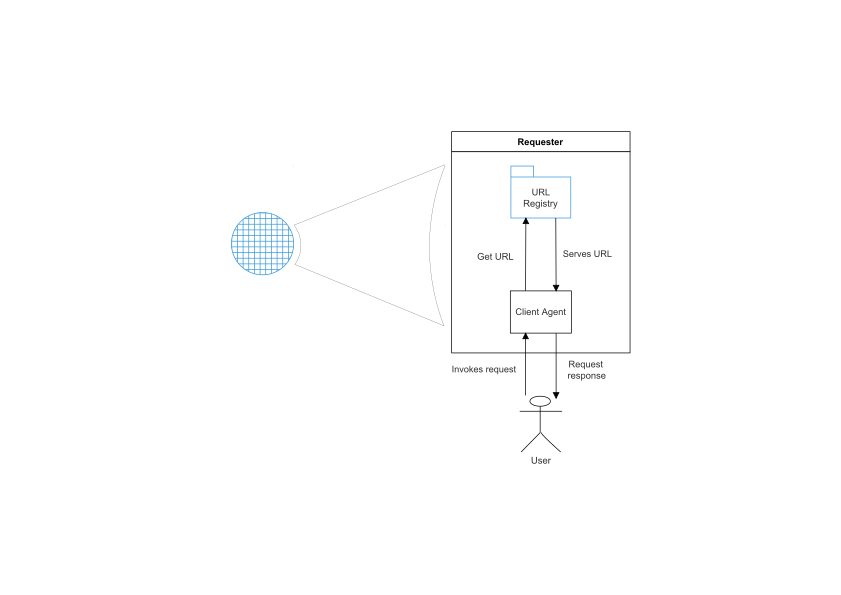
\includegraphics[width=14cm]{requester.jpg}
%  \caption{Requester}
%  \label{fig:requester}
%\end{figure}		
		
		\subsubsection{Client Agent}

		\subsubsection{URL Registry}

	\subsection{Provider}

%\begin{figure}[!htp]
%  \centering
%  \includegraphics[width=14cm]{provider.jpg}
%  \caption{Provider}
%  \label{fig:provider}
%\end{figure}	


		\subsubsection{Server Agent}
		
		\subsubsection{Query Builder}
		
		\subsubsection{Mapper}
		

%\section{Service Layers Architecture}


%\begin{figure}[!htp]
%  \centering
%  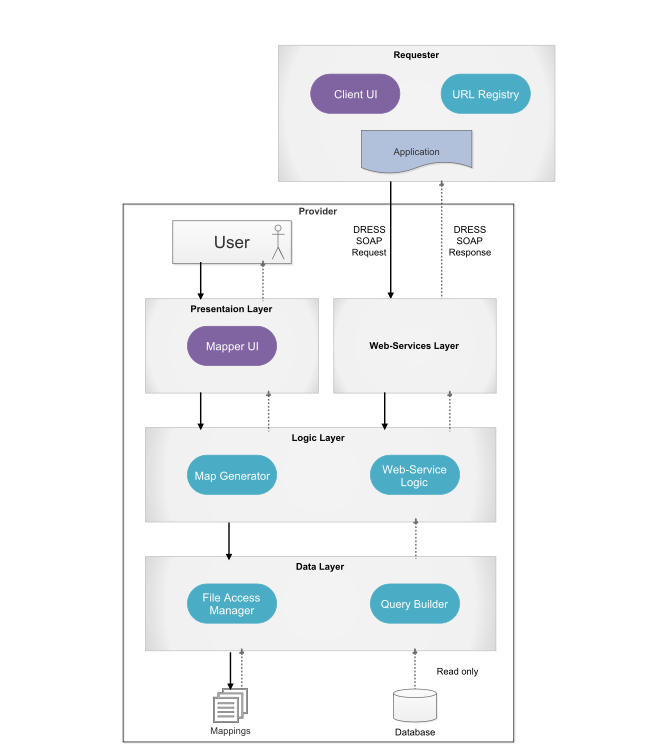
\includegraphics[width=14cm]{service_layers.jpg}
%  \caption{Service Layers Architecture Diagram}
%  \label{fig:architecture}
%\end{figure}


%%%%%%%%%%%%%%%%%%%%%%%%%%%%%%%%%%%%%%%%%%%%%%%%%%%%%%%%%%%

\chapter{Document Record Exchange Standard for Students}\label{ch-DRESS}

\chapter{Implementation \& Evaluation}\label{ch-implement}


\section{Implementation Stages}
Automating exchange of educational certificates using DRESS can be divided into four stages of implementation. The very first stage begins with defining the schema, that is our proposed standard and writing an XSD. The second stage involves implementation of a mapping tool that generates mapping and filters over heterogeneous schemas. The third stage is the development of a web-service that uses the generated mappings and filters to serve requests using DRESS. In this stage we implement a soap service describing the possible operations in a WSDL that satisfy the business processes described in chapter. The fourth stage is the last stage which includes development of a GUI interface for a Client which is a central authority to send and retrieve information from different institutes/nodes.
 
\subsection{Defining the Schema}
DRESS defines vocabulary for educational certificates. Using this vocabulary, XML documents are created for the exchange of documents to take place. There are different types of documents like DEGREE, REGISTRATION and TRANSCRIPT. Each document has a corresponding XML document. At this stage we create the XSDs for these XML documents.

\subsection{Map Generation}
Using the defined schema, we create mappings at stage 2. A semi-automated wizard is run on the provider node to create mappings and filters. These mappings and filters are stored in JSON format as properties.  The Mapping Tool and generated mappings reside on the provider node.

\subsection{DRESS based Web-Service}
At stage 3, a SOAP based web-service uses the defined mappings and filters. This piece of code fetches data from the provider database using the mappings. The fetched data is then served in DRESS format to the  request/client. The SOAP base web-service runs on the provider node. 

\subsection{Client}
At stage 4, a request mechanism is developed on the central Authority. A client tool is developed that enables us to request the DRESS based web-services using a graphical user interface. It then displays the exchanged document in readable format.

\section{Tools \& Technologies}
In this section, we discuss some important implementation decisions, and the technologies we chose for implementation. These decisions are based on following concerns;

\begin{enumerate}

\item The tools we developed will be freely available, so we choose to use open-source technologies as much as possible.

\item The implementation and deployment involves many parties. For example, every institute has to use our mapping tool to generate mappings. This piece of software must be easy to use and should be able to run with zero configuration. Hence, we chose mappings to be stored as properties on the secure server disk in JSON format. This enables us to run this mapping wizard tool on a web-server with almost zero configuration.	

\end{enumerate}

\section{Evaluation}
In this section we present the evaluation techniques that can be used and the ones we used to evaluate this research against the target goals discussed in section \ref{s-goals}. We list down these techniques and later discuss these in detail.

	\begin{enumerate}

	\item Evaluating against functional \& non-functional requirements.

	\item Using program validation technique. \cite{Sieve}
	
	\item Fault-based testing of XML Schema.
	
	%\item Testing against exemplary data.
	
	%\item Success and failure statistics for different cases.	

	\end{enumerate}
	
	All the above mentioned techniques require us to create a test bed environment. Hence, we created an environment of three nodes for the evaluation purpose. \\
	
	\subsection{Test-bed}
	Keeping in mind the end goal to mimic a true domain and to simulate more realistically, it is better to setup separate servers for each node/entity. So we setup separate server for each node with different technologies and services running on these machines. We take three nodes as shown in figure ~\ref{fig:testbed}. The two nodes (Node1 with horizontal lines and Node2 with vertical lines) are the providers and the node (Node0 with grid pattern) in the center is the node that acts as a central authority. Both provider nodes are running database management systems and schema that are different from each other. Thus simulating a heterogeneous environment.
	
\begin{figure}[!htp]
  \centering
  \includegraphics{architecture_distributed_testbed_exchange_through_hec.jpg}
  \caption{Three Nodes Exchanging Information Usign DRESS with one Node as Central Control Authority}
  \label{fig:testbed}
\end{figure}  

We begin with setting up the providers first by generating mappings over the heterogeneous schema and then installing the web-services that enable these providers to exchange educational certificates. Once the providers are ready, we setup the client to use the provider web-services for exchanging information using DRESS.

	\begin{enumerate}  

		\item At Node1, we installed MS-SQL as database management system with a university database schema. We generated mappings using the mapping tool and then setup the DRESS based provider web-service.

		\item At Node2, we installed MySQL as database management system with another university documents  database. We generated mappings for this schema and then setup the DRESS based provider web-service. 
	
		\item At Node0, we installed the client GUI which enables us to request information regrading educational certificates from the providers. 

	\end{enumerate}
	
It is worth mentioning that the mappings generated at Node1 and Node2 are different and correspond to their respective schema only. 

	\subsection{Evaluation Techniques}
	We discuss the evaluation techniques that can be used for evaluating our proposed standard and the proposed architecture. We also provided references of the research projects where these techniques have already been used as an example. We apply these techniques to evaluate against the goals we discussed in sections \ref{s-goals}. 
	
	% We apply these techniques to evaluate against the goals and challenges we discussed in sections \ref{s-goals} and \ref{s-challenges} respectively. \\
	
		\subsubsection{Evaluating against Functional \& Non-Functional Requirements}
		We listed functional and non-functional requirements in section \ref{s-softspecs} for achieving the goals mentioned in section \ref{s-goals}.  In this technique we subjectively evaluate these requirements. Let us begin with functional requirements first.
		% and meeting the challenges explained in section \ref{s-challenges}
	\begin{enumerate}  

		\item Starting with first functional requirement, we can express that the proposed architecture and DRESS based effective information trade of educational certificates between partaking institutes in the test-bed environment. This worked successfully for the different heterogeneous schema running on different database engines. 

		\item The test-bed also satisfied the second requirement and only provider data is only shared if a request is made with valid access keys. 
	
		\item We collected real educational certificates and added this record to two different test schema on each node. We see that the system is testable with this data. Hence, we met this third requirement.
		
		\item We added two new providers in the environment in a semi-automated way to generate mappings using the mapping tool and made agreements. This satisfies the fourth requirement.

	\end{enumerate}
		
	We now evaluate the non-functional requirements which are relatively hard to measure. A subjective evaluation of the non-functional requirements is below;
	
	\begin{enumerate}  

		\item We exchanged different documents and similar documents from different issuing authorities with a few changes at attribute level. However, it is hard to test with every possible document but we were able to test the standard for documents from different issuing authorities. These document contained differences at attribute level and among values. For example, the grade and mark attributes are used both with divisions plus percentage and grades plus CGPA. This successful exchange satisfies the non-functional requirement number 1.

		\item The architecture is designed in such a way that it provides both control and authority. The only authority that may request data from the providers in this architecture is the Node0 (the central authority). This satisfies the non-functional requirement number 2. 
	
		\item Both providers Node1 and Node2 in the test-bed are the owner of their data. Providers are autonomous bodies approved from a central authority. Since, the data is not copied to some other authority and a document exchange request is always made to the corresponding provider. For example, University 1 at Node1 will always serve exchange requests for its documents and every time request is made to Node1. This makes University1 owner of its own data and thus builds trust in the system. This satisfies the third requirement.
		
		\item The mapping tool made it easy to integrate new providers into the system in a semi-autmated way. This satisfies the fourth requirement. 
		
		\item We used open-source technologies that are widely used for setting up test-bed. We used JSON for storing mappings which require no storage configurations. We used PHP as server-side programming language for the development of the web-service and the query builder. HTML and JavaScript are used for front end development. All the technologies are openly available, free and widely used. This satisfies the fifth requirement.

	\end{enumerate}
		
		
		\subsubsection{Using Program Validation Technique}
		Program validation technique unit testing and integration testing of the tools that are developed. This technique reports the issues and bugs found in the developed tools. However, in this research our focus is on our proposed standard DRESS and the proposed architecture. Although we developed software tools to evaluate DRESS and the architecture but the testing of the these tools itself is out of scope of this research. 
		
		\subsubsection{Using Fault-based Testing}
		We used this evaluating technique to test the XML schema for detecting faults. Starting with the creation of a formal model for the schema under consideration, we create fault classes. These fault classes are used to generate the queries. We run these queries against the test-data. The test data are the sniffed XML documents while exchange between during partaking institutes. The results of the queries are then compared with the specified schema to detect faults. The testing process we followed is shown in figure~\ref{fig:fault-based-testing}. It should be noted that instead of mutating the data, we sniffed the traffic and used the captured XML documents as test-data.  		
		
\begin{figure}[!htp]
  \centering
  \includegraphics[width=13.5cm]{fault-based-testing.jpg}
  \caption{Testing process for detecting faults}
  \label{fig:fault-based-testing}
\end{figure}
		%\subsubsection{Testing against Exemplary data}
		%This technique involves running the system with different data-sets by different users and then getting feedback. We collected documents for two different 
	
		%\subsubsection{Success Vs Failure Cases}


%\subsection{Apache HTTP Server}

%\subsection{Codeigniter Framework}

%\subsection{PHP2WSDL}

%\subsection{MySQL}

\chapter{Conclusion \& Future Work}\label{ch:Conclusions}


	\section{Conclusion}\label{sec:conclusion}

	In this research we reported........ .

	\section{Future Work}\label{sec:future}
	Unified Measurements \cite{EHEA}
	
	Document Authentication \cite{Authentic PDF}
	
	Search Across Databases \cite{Search Across Space Databases}
	
	Become base of may automation projects like mobility.
	
	
	
	


%\backmatter


\begin{thebibliography}{10}

\bibitem{umair}
M. Ali, H. Qureshi, and M. S. Akhtar (2013), \emph{Analysis of growth in Students Intake and Degree Awarding Contribution: A Comparison of Stanford and MIT}, MLDM 2013: International Conference on Machine Learning and Data Mining, in press.

\bibitem{bologna process}
http://www.ehea.info/Uploads/Irina/Bologna%20beyond%202010.pdf

\bibitem{MAPQFTOOL}
P. Pouyioutas, H. Gjermundrod, and M. Michael, "MAPQFTOOL: A software tool to support national qualifications frameworks," Information Society (i-Society), 2011 International Conference on, pp. 198-203, Jun. 2011.

\bibitem{The Mobility Project}
Rafal Nagrodzki, "The Mobility Project," Institue of Informatics, University of Warsaw, Warsaw, Master's Thesis 2009.

\bibitem{EHEA}
A. Duran, Y.B. Moon, and E. Giraldo, "Work in progress - the European Higher Education Area ("Bologna process") in Engineering Education in Spain," Frontiers in Education Conference, 2009. FIE '09. 39th IEEE, pp. 1,2, Oct. 2009.

\bibitem{Integration of Services in the Mobility Project}
Karol Kanski, "Integration of Services in the Mobility Project," Institute of Informatics, University of Warsaw, Warsaw, Master's Thesis 2011.

\bibitem{Data integration: the teenage years}
Alon Halevy, Anand Rajaraman, and Joann Ordille, "Data integration: the teenage years," In Proceedings of the 32nd international conference on Very large data bases (VLDB '06), pp. 9-16, 2006.

\bibitem{improvement bologna process}
Szentirmai, L.; Radacs, L., "Improvement of academic and research standards of higher engineering education in light of Bologna process," Emerging eLearning Technologies \& Applications (ICETA), 2012 IEEE 10th International Conference on , vol., no., pp.381,386, 8-9 Nov. 2012

\bibitem{SCHAC 1.5.0}
https://wiki.refeds.org/download/attachments/1606048/SCHAC
\%2B1.5.0.pdf?version=3\&modificationDate=1429195142624\&api=v2

\bibitem{Edu Stat}
http://www.aepam.edu.pk/files/educationstatistics/pakistaneducation
statistics2010-11.pdf

\bibitem{Edu Stat2}
http://www.aepam.edu.pk/files/educationstatistics/pakistaneducation
statistics2013-14.pdf

\bibitem{Level of Edu}
http://www.pbs.gov.pk/sites/default/files//tables/POPULATION BY LEVEL OF EDUCATION AND SEX.pdf

\bibitem{Europass Web}
https://europass.cedefop.europa.eu/en/home

\bibitem{Authentic PDF}
Neubauer, T.; Weippl, E.; Biffl, S., "Digital signatures with familiar appearance for e-government documents: authentic PDF," Availability, Reliability and Security, 2006. ARES 2006. The First International Conference on , vol., no., pp.8 pp.,, 20-22 April 2006

\bibitem{Search Across Space Databases}
Maluf, D.A.; McDermott, W.J.; Knight, C.D.; Smith, E.E.; Gurram, M., "Searching Across the International Space Station Databases," Aerospace Conference, 2007 IEEE , vol., no., pp.1,8, 3-10 March 2007

\bibitem{Sieve}
http://hdl.handle.net/1721.1/27091


\end{thebibliography}

\end{document} 